% Project proposal: pattern-agnostic multispectral demosaicking.
% Based on the ICIP-2026 template; to be used with:
%          spconf.sty  - ICASSP/ICIP LaTeX style file, and
%          IEEEbib.bst - IEEE bibliography style file.
% --------------------------------------------------------------------------
\documentclass{article}
\usepackage{spconf,amsmath,amssymb,graphicx,tikz,url,array}
\newcolumntype{L}[1]{>{\raggedright\arraybackslash}p{#1}}
\usetikzlibrary{arrows.meta,positioning}

% Notation.
% ---------
\def\X{{\mathbf X}}
\def\Y{{\mathbf Y}}
\def\C{{\mathbf C}}
\def\M{{\mathbf M}}
\def\N{{\mathbf N}}
\def\x{{\mathbf x}}

% Spectral palette used to draw the MSFA patterns (band 1 = violet, 16 = red).
\definecolor{b1}{HTML}{5B3FD0}\definecolor{b2}{HTML}{4F4FD8}
\definecolor{b3}{HTML}{3F62DC}\definecolor{b4}{HTML}{2A75DB}
\definecolor{b5}{HTML}{1E88D0}\definecolor{b6}{HTML}{1A99B8}
\definecolor{b7}{HTML}{1BA49B}\definecolor{b8}{HTML}{2DAE7A}
\definecolor{b9}{HTML}{5BB55A}\definecolor{b10}{HTML}{8FBC40}
\definecolor{b11}{HTML}{C2C036}\definecolor{b12}{HTML}{E3B935}
\definecolor{b13}{HTML}{E8A030}\definecolor{b14}{HTML}{E8822C}
\definecolor{b15}{HTML}{DD5E31}\definecolor{b16}{HTML}{C93A3A}

% \msfa{expr}: draws a 16x16 crop of an MSFA; expr gives the band (1..16)
% of the pixel in row \i and column \j (both 0-based).
\newcommand{\msfa}[1]{%
  \begin{tikzpicture}[x=0.16cm,y=0.16cm]
    \foreach \i in {0,...,15}{
      \foreach \j in {0,...,15}{
        \pgfmathtruncatemacro{\b}{#1}
        \edef\c{b\b}
        \fill[fill=\c] (\j,-\i) rectangle ++(1,-1);
      }
    }
    \draw[black!60, line width=0.3pt] (0,0) rectangle (16,-16);
  \end{tikzpicture}}

% Title.
% ------
\title{PATTERN-AGNOSTIC MULTISPECTRAL DEMOSAICKING:\\
  BACKGROUND AND PROJECT PROPOSAL}
%
% Two authors, same affiliation (replace the placeholders).
% ----------------------------------------------------------
\name{{[Author One]}, {[Author Two]}}
\address{{[Course: Computational Photography 2026-2]}\\
  {[Department, University]}\\
  {[City, Country]}}
%
\begin{document}
%
\maketitle
%
\begin{abstract}
Snapshot multispectral cameras place a multispectral filter array (MSFA) over
the sensor, so each pixel measures only one of $L$ spectral bands and the
missing $(L-1)/L$ of the datacube must be recovered by demosaicking. This
document first reviews the background of the problem: multispectral image
formation, MSFA design (including recent designs based on optimal sphere
packing), classical and learned demosaicking, and the usual datasets and
metrics. Learned demosaicking currently gives the best reconstructions, but
each network is trained for one specific MSFA and must be retrained whenever
the filter pattern changes. We then propose a six-week project to study a
\emph{pattern-agnostic} network: a small U-Net that receives both the raw
mosaic and the MSFA mask, and is trained on randomly sampled patterns. We
describe the evaluation on seen and unseen MSFAs, and three levels of scope
that fit the available time.
\end{abstract}
%
\begin{keywords}
Multispectral imaging, multispectral filter array, demosaicking, deep
learning, generalization
\end{keywords}
%
\section{Introduction}
\label{sec:intro}

A conventional color camera records three values per pixel (red, green and
blue), which roughly match the three types of cone cells in the human eye.
Most materials, however, have spectral signatures with much more detail than
three numbers can describe. Multispectral imaging (MSI) records the scene in
several narrow spectral bands, typically between 8 and 32 in the visible and
near-infrared range. The result is a 3D \emph{datacube} with two spatial
dimensions and one spectral dimension. Because the spectrum at each pixel
helps to identify materials that look alike in RGB, MSI is used in remote
sensing to classify vegetation, soil and buildings~\cite{diaz2023}, in
medicine to analyze tissue and detect tumors~\cite{lu2014}, and in
agriculture, food inspection and cultural heritage.

The main difficulty of MSI is acquisition. A 2D sensor cannot record a 3D
datacube in one exposure without some trade-off. Snapshot cameras based on a
\emph{multispectral filter array} (MSFA) accept a loss of spatial sampling: a
mosaic of narrow-band filters is placed over the sensor, and each pixel
measures a single band~\cite{lapray2014}. The missing values must then be
estimated by a \emph{demosaicking} algorithm. With $L=16$ bands, each band is
measured at only $1/16$ of the pixels, so about 94\% of the datacube must be
estimated. This is far more difficult than RGB demosaicking, where the green
channel is measured at half of the pixels.

This document has two goals. Sections~\ref{sec:msi}--\ref{sec:eval} provide
a complete background on the problem, so that the reader can understand the
state of the art and its limitations. Sections~\ref{sec:gap}--\ref{sec:plan}
present our project proposal, which addresses one open problem: the
dependence of learned demosaicking networks on a specific MSFA pattern.

\section{Multispectral image acquisition}
\label{sec:msi}

\subsection{The multispectral datacube}

We denote the datacube by $\X\in\mathbb{R}^{H\times W\times L}$, where
$H\times W$ is the spatial resolution and $L$ is the number of bands. The
$k$-th band $\X_k\in\mathbb{R}^{H\times W}$ is a grayscale image of the scene
seen through a narrow filter centered at wavelength $\lambda_k$, and the
vector $\x(m,n)\in\mathbb{R}^L$ is the spectrum at pixel $(m,n)$. Natural
multispectral images have two strong forms of redundancy that every
reconstruction method exploits: \emph{spatial correlation} (neighboring pixels
tend to have similar values) and \emph{spectral correlation} (bands with close
central wavelengths look very similar, and their differences are smoother than
the bands themselves).

\subsection{Scanning and snapshot cameras}

Traditional spectral cameras scan the datacube. Whiskbroom and pushbroom
systems scan it spatially, one point or one line at a time, and tunable-filter
systems scan it spectrally, one band at a time~\cite{lapray2014}. Scanning
gives full resolution, but it is slow, needs complex hardware and fails with
moving scenes. \emph{Snapshot} cameras capture all the information in a single
exposure. One family uses coded apertures and dispersive optics followed by
a compressive reconstruction, such as the coded aperture snapshot spectral
imager (CASSI)~\cite{arce2014}. MSFA cameras are a simpler alternative: they
need no extra optics, are compact and inexpensive, and work in real time.
Their cost is the subsampling described above.

\subsection{From color filter arrays to MSFAs}

The Bayer color filter array~\cite{bayer1976} repeats a $2\times2$ kernel with
two green, one red and one blue filter. An MSFA generalizes this idea to $L$
narrow-band filters arranged in a $P\times P$ kernel that is repeated over the
whole sensor (Fig.~\ref{fig:patterns}). For example, commercial IMEC sensors
use $4\times4$ kernels with 16 bands and $5\times5$ kernels with 25
bands~\cite{geelen2014}. When every band appears once per kernel, each band
is sampled at $1/L$ of the pixels; some designs repeat a ``dominant'' band to
sample it more densely, at the cost of the other bands~\cite{miao2006}.
Real filters are not ideal: each one has a broad spectral response that
overlaps with its neighbors (crosstalk), which further mixes the bands.

\subsection{Image formation model}

Let $\C_k\in\{0,1\}^{H\times W}$ be the binary mask of band $k$, with
$\C_k(m,n)=1$ if pixel $(m,n)$ carries the filter of band $k$, and
$\sum_k\C_k=\mathbf{1}$ (every pixel has exactly one filter). Assuming ideal
narrow-band filters, the sensor records a single grayscale mosaic
\begin{equation}
  \Y = \sum_{k=1}^{L} \X_k \odot \C_k + \N,
  \label{eq:model}
\end{equation}
where $\odot$ is the element-wise product and $\N$ is sensor noise. This is
the discrete model used in~\cite{diaz2023}. We also define the one-hot mask
$\M=[\C_1,\dots,\C_L]\in\{0,1\}^{H\times W\times L}$, which fully describes
the MSFA. With real filters, each $\C_k$ becomes a weighted, non-binary
response.

\section{The demosaicking problem}
\label{sec:demosaicking}

Demosaicking computes an estimate $\hat\X$ of the full datacube from the
mosaic $\Y$. The problem is severely ill-posed: Eq.~\eqref{eq:model} provides
$HW$ measurements for $HWL$ unknowns, so it has infinitely many solutions.
Every method must therefore add prior knowledge about natural images, usually
spatial and spectral correlation. When the prior fails, three typical
artifacts appear~\cite{diaz2023}:
\begin{itemize}
  \item \textbf{Zipper effect:} alternating errors along edges, which follow
        the periodic structure of the filter kernel.
  \item \textbf{False colors:} spectra that do not exist in the scene,
        produced when bands are interpolated inconsistently near edges.
  \item \textbf{Blur:} loss of fine textures caused by interpolating each
        band from very sparse samples.
\end{itemize}

\subsection{Classical methods}

\textbf{Weighted bilinear (WB) interpolation.} Brauers and
Aach~\cite{brauers2006} interpolate each sparse band $\X_k\odot\C_k$
independently with a normalized low-pass kernel. WB is simple and fast, but
it ignores spectral correlation and produces strong blur.

\textbf{Spectral-difference methods.} Instead of interpolating a band
directly, these methods interpolate the difference between two bands, which
is smoother. Spectral difference (SD)~\cite{brauers2006} estimates band $k$ at
a pixel of band $l$ by interpolating $\X_k-\X_l$, and iterative spectral
difference (ItSD)~\cite{mizutani2014} repeats the estimation and gives more
weight to bands with close central wavelengths, which are more correlated.

\textbf{Intensity- and panchromatic-guided methods.} A second family first
estimates an image that contains information from all bands and uses it as a
guide. Intensity difference (ID) interpolates the differences between each
band and an estimated intensity image; iterative variants refine the intensity
estimate (ItID), or compute it only from the spectrally nearest channels
(ItNCD), which gives the best classical results in~\cite{diaz2023}. The
pseudo-panchromatic image difference (PPID)~\cite{mihoubi2017} estimates the
average of all bands directly from the mosaic and interpolates the
differences between each band and this pseudo-panchromatic image.

\textbf{Optimization methods.} Demosaicking can also be written as a
regularized inverse problem. For example, Tsagkatakis et
al.~\cite{tsagkatakis2019} recover IMEC mosaics with low-rank and graph
regularization.

\subsection{Learned methods}

Convolutional neural networks learn the prior directly from training data.
Given pairs $(\Y,\X)$ simulated with Eq.~\eqref{eq:model}, a network
$f_\theta$ is trained to minimize a loss such as
$\|f_\theta(\Y)-\X\|_1$. Examples include the mosaic convolution-attention
network (MCAN)~\cite{feng2021} and TRevSCI~\cite{diaz2023}, which adapts the
RevSCI architecture for snapshot compressive imaging~\cite{cheng2021} to MSFA
demosaicking. For RGB cameras, Gharbi et al.~\cite{gharbi2016} showed that
demosaicking and denoising are better solved jointly by a single network.

Learned methods outperform classical ones in both spatial and spectral
fidelity~\cite{diaz2023}. However, the network usually receives only $\Y$, so
it learns the pattern \emph{implicitly}, and its parameters become tied to
the MSFA used during training. In~\cite{diaz2023}, TRevSCI was retrained for
every pattern, and each training took about a day and a half on two GPUs.

\section{MSFA design and optimal sphere packing}
\label{sec:design}

The demosaicking quality also depends on where each filter is placed.
Classical MSFAs are designed ad hoc: random permutations (RND), sequential
arrangements (SEQ), the Brauers--Aach pattern (BRA)~\cite{brauers2006},
the binary-tree-based edge-sensing pattern (BTES)~\cite{miao2006} and the IMEC
mosaics~\cite{geelen2014}. Hirakawa and Wolfe~\cite{hirakawa2008} proposed
one of the first mathematical criteria, based on the Fourier domain, for color
filter arrays.

Diaz et al.~\cite{diaz2023} recently proposed a geometric criterion, called
MSFA by optimal sphere packing (MSFA-OSP). Each sampled pixel is represented
by its coordinates (row, column, band) inside a discrete
$L\times L\times L$ spatio-spectral cube. A good MSFA should sample this cube
uniformly, which means that the sampled points should be as far apart as
possible. If a sphere of equal size is centered at each point, the design
becomes a \emph{sphere packing} problem: maximize the minimum distance
between centers, so that the spheres are as large as possible without
overlapping. By Kepler's conjecture, no packing of equal spheres in 3D is
denser than the face-centered cubic lattice, whose density is
$\pi/\sqrt{18}\approx0.74$; this gives an upper bound for the
design~\cite{diaz2023}.

Because a sensor imposes a discrete grid, the authors restrict the search to
patterns of the form
\begin{equation}
  B = \big((a\,I + b\,J)\bmod L\big) + 1,
  \label{eq:osp}
\end{equation}
where $I$ and $J$ are the row and column index matrices of an $L\times L$
kernel, and $a,b$ are integers. An algorithm evaluates the candidate pairs
$(a,b)$ with $a,b\le\lfloor L/2\rfloor$, keeps those with a uniform number of
filters, and selects the pair with the largest minimum distance. The optimal
values are $a=7$, $b=4$ for $L=16$ and $a=8$, $b=3$ for $L=25$, and they are
computed in less than half a second, whereas blue-noise designs may take
several minutes~\cite{diaz2023}.

Table~\ref{tab:sp} summarizes the reported geometry. OSP achieves the largest
sphere diameter and packing density, and the authors report up to 2\,dB of
PSNR improvement over seven state-of-the-art MSFAs, together with fewer
zipper and false-color artifacts~\cite{diaz2023}. In our project, the MSFA is
an experimental variable, and we use OSP as one of the test patterns.

\begin{figure}[htb]
\centering
\begin{minipage}[b]{0.32\linewidth}
  \centering
  \msfa{{7,8,6,5,15,16,14,13,11,12,10,9,3,4,2,1}[4*mod(\i,4)+mod(\j,4)]}
  \centerline{(a) IMEC}
\end{minipage}
\hfill
\begin{minipage}[b]{0.32\linewidth}
  \centering
  \msfa{{1,13,4,15,9,5,11,7,3,16,2,14,12,8,10,6}[4*mod(\i,4)+mod(\j,4)]}
  \centerline{(b) BTES}
\end{minipage}
\hfill
\begin{minipage}[b]{0.32\linewidth}
  \centering
  \msfa{mod(7*(\i+1)+4*(\j+1),16)+1}
  \centerline{(c) OSP}
\end{minipage}
\caption{$16\times16$ crops of three MSFAs with $L=16$ bands (color = band,
from violet to red). (a) IMEC $4\times4$ kernel~\cite{geelen2014}; (b)
BTES~\cite{miao2006}; (c) sphere-packing pattern of Eq.~\eqref{eq:osp} with
$a=7$, $b=4$~\cite{diaz2023}. Patterns (a) and (b) are taken from the public
code of~\cite{diaz2023}.}
\label{fig:patterns}
\end{figure}

\begin{table}[htb]
\centering
\caption{Sphere diameter $d$ and packing density $\rho$ of MSFAs with $L=16$,
as reported in~\cite{diaz2023}. Higher values mean more uniform sampling.}
\label{tab:sp}
\footnotesize
\begin{tabular}{|l|c|c|}
\hline
MSFA & $d$ & $\rho$ \\
\hline
RND                          & 1.00 & 0.03 \\
BN, BRA, SEQ, UNIF, IMEC      & 1.41 & 0.08 \\
BTES                         & 1.73 & 0.14 \\
OSP                          & 2.45 & 0.40 \\
\hline
\end{tabular}
\end{table}

\section{Datasets and evaluation}
\label{sec:eval}

\textbf{Datasets.} Because ground-truth datacubes cannot be captured with an
MSFA camera, research on demosaicking uses datacubes from scanning cameras and
simulates the mosaic with Eq.~\eqref{eq:model}. The CAVE
dataset~\cite{yasuma2010} contains 32 indoor scenes of $512\times512$ pixels
with 31 bands from 400 to 700\,nm in 10\,nm steps, and is the usual test set.
Larger datasets for training include TokyoTech~\cite{monno2015}, ICVL, Harvard
and ARAD-1K~\cite{arad2022}, which contains about one thousand scenes with 31
bands.

\textbf{Metrics.} Spatial fidelity is measured with the peak signal-to-noise
ratio,
\begin{equation}
  \mathrm{PSNR} = 10\log_{10}\frac{v_{\max}^2}{\frac{1}{HWL}\|\hat\X-\X\|_2^2},
\end{equation}
where $v_{\max}$ is the maximum value of the data, and with the structural
similarity index (SSIM)~\cite{wang2004}, averaged over bands. Spectral
fidelity is measured with the spectral angle mapper~\cite{kruse1993},
\begin{equation}
  \mathrm{SAM} = \frac{1}{HW}\sum_{m,n}\arccos
  \frac{\langle \x(m,n),\hat\x(m,n)\rangle}{\|\x(m,n)\|\,\|\hat\x(m,n)\|},
\end{equation}
the average angle between the true and estimated spectra. Higher PSNR and SSIM
and lower SAM indicate better reconstructions.

\section{Open problem and research question}
\label{sec:gap}

The background shows that the two levers of MSFA imaging have advanced
separately. Pattern design now has a principled criterion (OSP), and learned
networks give the best reconstructions. However, learned networks are tied to
the pattern used in training. The authors of~\cite{diaz2023} state that ``a
significant limitation of the proposed method is the necessity of retraining
for specific MSFAs'', and they leave the generalization to new MSFAs as
future work. This dependence is costly: comparing $n$ patterns requires
training $n$ networks, and a camera with a different or slightly defective
pattern needs a new model. To our knowledge, the generalization of learned
MSFA demosaicking across patterns has not been systematically evaluated.

Our research question is: \emph{can a single demosaicking network reconstruct
multispectral images from any MSFA, including patterns not seen during
training, with a quality close to that of a network trained for each
pattern?} Our objectives are:
\begin{enumerate}
  \item Build an open Python simulation pipeline (patterns, acquisition model,
        metrics) and classical baselines.
  \item Quantify how much a pattern-specific network degrades on unseen MSFAs.
  \item Propose and evaluate a mask-conditioned network trained on random
        patterns.
\end{enumerate}

\section{Proposed method}
\label{sec:method}

\textbf{Mask-conditioned network.} We give the pattern to the network as an
explicit input. The network receives the mosaic $\Y$ together with the
one-hot mask $\M$ and computes $\hat\X=f_\theta(\Y,\M)$
(Fig.~\ref{fig:method}). By default, the input is the concatenation
$[\Y,\M]$; as an extension, we will compare it with the sparse cube
$\Y\odot\M$, which places each measured value in its own band. The backbone is
a small
U-Net~\cite{ronneberger2015} with fewer than two million parameters, trained
with the $\ell_1$ loss used in~\cite{diaz2023}.

\textbf{Training on random patterns.} If a network is always trained with the
same MSFA, it can ignore $\M$ and memorize the pattern. Therefore, for each
training batch we sample a new random \emph{valid} pattern, that is, a random
assignment of bands within a $P\times P$ kernel in which every band appears the
same number of times, and simulate the mosaic with Eq.~\eqref{eq:model}. This
forces the network to read the mask. The structured patterns of
Fig.~\ref{fig:patterns} are never used in training, so they are unseen at test
time.

\begin{figure}[htb]
\centering
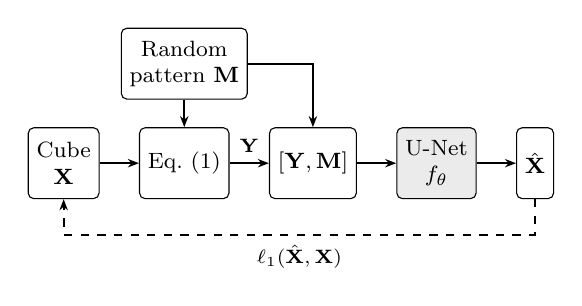
\begin{tikzpicture}[
    box/.style={draw, rounded corners=2pt, align=center, minimum height=0.9cm,
                font=\footnotesize, inner sep=3pt},
    arr/.style={-{Stealth[length=4pt]}, thick}]
  \node[box] (cube) {Cube\\$\X$};
  \node[box, right=0.5cm of cube] (sim) {Eq.~(1)};
  \node[box, above=0.35cm of sim] (rand) {Random\\pattern $\M$};
  \node[box, right=0.5cm of sim] (in) {$[\Y,\M]$};
  \node[box, right=0.5cm of in, fill=black!8] (net) {U-Net\\$f_\theta$};
  \node[box, right=0.5cm of net] (out) {$\hat\X$};
  \draw[arr] (cube) -- (sim);
  \draw[arr] (rand) -- (sim);
  \draw[arr] (rand) -| (in);
  \draw[arr] (sim) -- node[above, font=\scriptsize] {$\Y$} (in);
  \draw[arr] (in) -- (net);
  \draw[arr] (net) -- (out);
  \draw[arr, dashed] (out.south) -- ++(0,-0.45) -| node[pos=0.25, below,
       font=\scriptsize] {$\ell_1(\hat\X,\X)$} (cube.south);
\end{tikzpicture}
\caption{Proposed training scheme. A new random MSFA $\M$ is sampled for each
batch, the mosaic $\Y$ is simulated with Eq.~(1), and the network receives
both $\Y$ and $\M$.}
\label{fig:method}
\end{figure}

\section{Experimental design}
\label{sec:experiments}

\textbf{Data.} We will train on a subset of 200--300 scenes of
ARAD-1K~\cite{arad2022}, keeping 10--15\% of them for validation, and
test on the 32 scenes of CAVE~\cite{yasuma2010},
as in~\cite{diaz2023}, so that training and test scenes come from different
datasets. As in~\cite{diaz2023}, we select 16 of the 31 bands. Training uses
$64\times64$ patches.

\textbf{Methods.} (1) Classical baseline: WB (PPID~\cite{mihoubi2017} only as an
extension). (2) Pattern-specific
networks: the same U-Net without the mask, trained only on IMEC or only on
OSP. (3) The proposed pattern-agnostic network.

\textbf{Metrics.} PSNR, SSIM and SAM (Section~\ref{sec:eval}), reported as
mean and standard deviation over the 32 CAVE scenes. We will also plot the
PSNR of each band against its wavelength and the spectral signatures of a few
selected pixels, and inspect zipper and false-color artifacts on zoomed
regions.

\textbf{Protocol.} Every method is evaluated on four test patterns
(Table~\ref{tab:protocol}). We will test three hypotheses:
\textbf{H1}: pattern-specific networks degrade strongly on unseen patterns;
\textbf{H2}: the agnostic network stays within 1\,dB of each specific network
on its own pattern; \textbf{H3}: the agnostic network clearly outperforms the
specific networks on unseen patterns.

\begin{table}[htb]
\centering
\caption{Evaluation protocol. ``Seen'': pattern used in training; ``unseen'':
pattern not used in training. Each cell will report PSNR / SSIM / SAM.}
\label{tab:protocol}
\footnotesize
\begin{tabular}{|l|c|c|c|c|}
\hline
Method $\backslash$ test MSFA & IMEC & OSP & BTES & Random \\
\hline
WB                & ref.   & ref.   & ref.   & ref.   \\
U-Net (IMEC)      & seen   & unseen & unseen & unseen \\
U-Net (OSP)       & unseen & seen   & unseen & unseen \\
Agnostic (ours)   & unseen & unseen & unseen & unseen \\
\hline
\end{tabular}
\end{table}

\textbf{Computing resources.} We do not have a dedicated GPU. Development and
short training runs will use an Apple M5 laptop (16\,GB, PyTorch with the MPS
backend), and longer runs will use free cloud GPU notebooks (e.g., Kaggle).
The small network, the small patches and the limited number of trained models
(three) keep the cost within this budget.

\section{Scope and work plan}
\label{sec:plan}

The project lasts six weeks, from October 5 to November 11, 2026, and is
carried out by two students, each with about six hours per week (roughly 65
person-hours in total). Student A is responsible for the data, the
simulator, the classical baselines and the evaluation; student B is
responsible for the networks. Both parts share one interface
(\texttt{simulate}, \texttt{method}, \texttt{evaluate}), so they can progress
in parallel.

\textbf{Scope levels.} We define three levels of scope; each level includes
the previous one (Table~\ref{tab:scope}). Level~A is guaranteed and already
answers H1. Level~B is our target; we estimate that it needs about 45--50
person-hours, which leaves a margin within our budget. For this reason, PPID
and the other extensions are left to level~C, which is only attempted if we
are ahead of schedule.

\begin{table}[htb]
\centering
\caption{Scope levels for the six-week project.}
\label{tab:scope}
\footnotesize
\begin{tabular}{|L{1.9cm}|L{5.9cm}|}
\hline
Level & Content \\
\hline
A: Minimum (end of week 3) &
  Simulator with 4 patterns; WB; IMEC-specific network; test on
  unseen patterns (H1). \\
\hline
B: Target (end of week 5) &
  A + agnostic network; OSP-specific network; full Table~\ref{tab:protocol}
  (H1--H3); per-band PSNR, spectral signatures and artifact analysis. \\
\hline
C: Extra (only if ahead) &
  B + PPID baseline; robustness to noise ($\N\neq 0$); real IMEC filter
  responses;
  comparison of the input encodings $[\Y,\M]$ and $\Y\odot\M$. \\
\hline
\end{tabular}
\end{table}

\textbf{Out of scope.} To keep the plan realistic, we will not capture data
with a real camera, reproduce TRevSCI or the full results
of~\cite{diaz2023}, design new MSFA patterns, or use more than 16 bands. These
topics can be discussed as future work.

\textbf{Timeline.} Table~\ref{tab:timeline} shows the weekly plan for
level~B. All experiments finish in week~5, so that week~6 is reserved for the
report and the presentation.

\begin{table}[htb]
\centering
\caption{Weekly plan (level B), with the tasks of each student.}
\label{tab:timeline}
\footnotesize
\begin{tabular}{|c|L{1.65cm}|L{2.4cm}|L{2.4cm}|}
\hline
Wk. & Dates & Student A & Student B \\
\hline
1 & Oct 5--11 & Data, simulator, metrics & PyTorch setup, U-Net, training loop \\
\hline
2 & Oct 12--18 & WB on CAVE & IMEC-specific network \\
\hline
3 & Oct 19--25 & Evaluation on 4 patterns (H1) & Agnostic network \\
\hline
4 & Oct 26--Nov 1 & OSP-specific network & Agnostic network (tuning) \\
\hline
5 & Nov 2--8 & \multicolumn{2}{L{5.2cm}|}{Full Table~\ref{tab:protocol} and
  artifact analysis (both)} \\
\hline
6 & Nov 9--11 & \multicolumn{2}{L{5.2cm}|}{Report and presentation (both)} \\
\hline
\end{tabular}
\end{table}

\textbf{Milestones.} (1) October 16: the full pipeline runs end to end, with
WB and the IMEC-specific network. (2) October 23: decision point; if the
IMEC-specific network works and H1 is measured, we continue to level~B,
otherwise we close the project at level~A. (3) November 6: experiments are
frozen and no new experiments are added. (4) November 11: final delivery
(report, presentation and code repository).

\textbf{Risks.} Since each student has about six hours per week, long
training runs will run unattended on cloud GPUs. If training is still too
slow, we will use fewer training scenes or smaller patches. If ARAD-1K is not available in time, we
will use cross-validation on CAVE (24 training and 8 test scenes). If the
agnostic network does not generalize, the project will still report and
analyze how strongly learned demosaicking depends on the pattern. A general
delay is handled by the decision point of October 23.

\section{Expected outcomes}
\label{sec:conclusion}

The project will deliver (i) an open Python pipeline for simulated MSFA
demosaicking, (ii) a measurement of how much pattern-specific networks
degrade on unseen MSFAs, and (iii) a single mask-conditioned network
evaluated on four different patterns. A positive result would remove the
need to retrain the network for each MSFA, which is the limitation reported
in~\cite{diaz2023}. A negative result would still be informative, because it
would quantify the cost of pattern dependence and motivate future work.

% References.
% -----------
\bibliographystyle{IEEEbib}
\bibliography{strings,refs}

\end{document}
